\section{Systemarchitektur und Rahmenbedingungen}

Die Konzeption eines Empfehlungssystems für den produktiven Einsatz bei der SV-Gruppe erfordert eine Architektur, die klar definierten Rahmenbedingungen gerecht wird. 
Aus dem Anwendungsfall ergeben sich eine Reihe von \ac{NFR}s, die die technische Ausgestaltung maßgeblich beeinflussen.

\subsection{Primäre nicht-funktionale Anforderungen}
\label{sec:nfr}
Für den initialen Proof-of-Concept wurden drei zentrale NFRs als erfolgskritisch identifiziert. 
Erstens muss das System eine hohe Performanz aufweisen und in der Lage sein, eine große Anzahl paralleler Anfragen effizient zu verarbeiten. 
Als konkretes \ac{SLO} wird eine 95-Perzentil-Latenz von unter 500 Millisekunden angestrebt. 
Zweitens ist die Skalierbarkeit der Architektur essenziell, um flexibel auf wachsende Nutzerzahlen und Datenmengen reagieren zu können, 
wie sie im dynamischen Umfeld eines Nachrichtenportals zu erwarten sind. Drittens muss eine einfache Integrierbarkeit gewährleistet sein, 
weshalb das System über eine standardisierte REST-API angebunden wird, um die Integration in bestehende Redaktions- und IT-Workflows zu erleichtern.

\subsection{Sekundäre und zukünftige Anforderungen}
Obwohl es sich zunächst um einen Prototypen handelt, wurden weitere Anforderungen identifiziert, die für einen späteren, 
vollumfänglichen Produktivbetrieb relevant sind. Dazu gehören die Gewährleistung von Datenschutz und Sicherheit gemäß der \ac{DSGVO}, 
eine hohe Verfügbarkeit und Ausfallsicherheit zur Sicherstellung eines unterbrechungsfreien Betriebs sowie die Transparenz der Empfehlungslogik, 
um das Vertrauen der Nutzer zu fördern. Diese Aspekte wurden im aktuellen Entwurf bereits konzeptionell berücksichtigt.

\subsection{Rahmenbedingungen}

Die bestehende IT-Infrastruktur der SV-Gruppe, die auf der \ac{GCP} basiert, definiert die zentralen Rahmenbedingungen für dieses Projekt. 
Der gesamte Artikelkorpus sowie die aus \ac{GA4} stammenden Nutzerinteraktionsdaten liegen zentral in BigQuery-Tabellen vor. 
Eine entscheidende und bereits vorhandene Ressource stellen hochdimensionale (3072D) Artikel-Embeddings dar, 
welche aus den Titeln und Texten der Artikel generiert wurden. Aufgrund ihrer bewährten Effektivität in verwandten Anwendungsfällen, 
wie der semantischen Anzeigenausspielung, werden diese Embeddings auch im Rahmen dieser Arbeit genutzt.

\subsection{Technologische Architektur}
\begin{figure}[htbp]
    \centering
    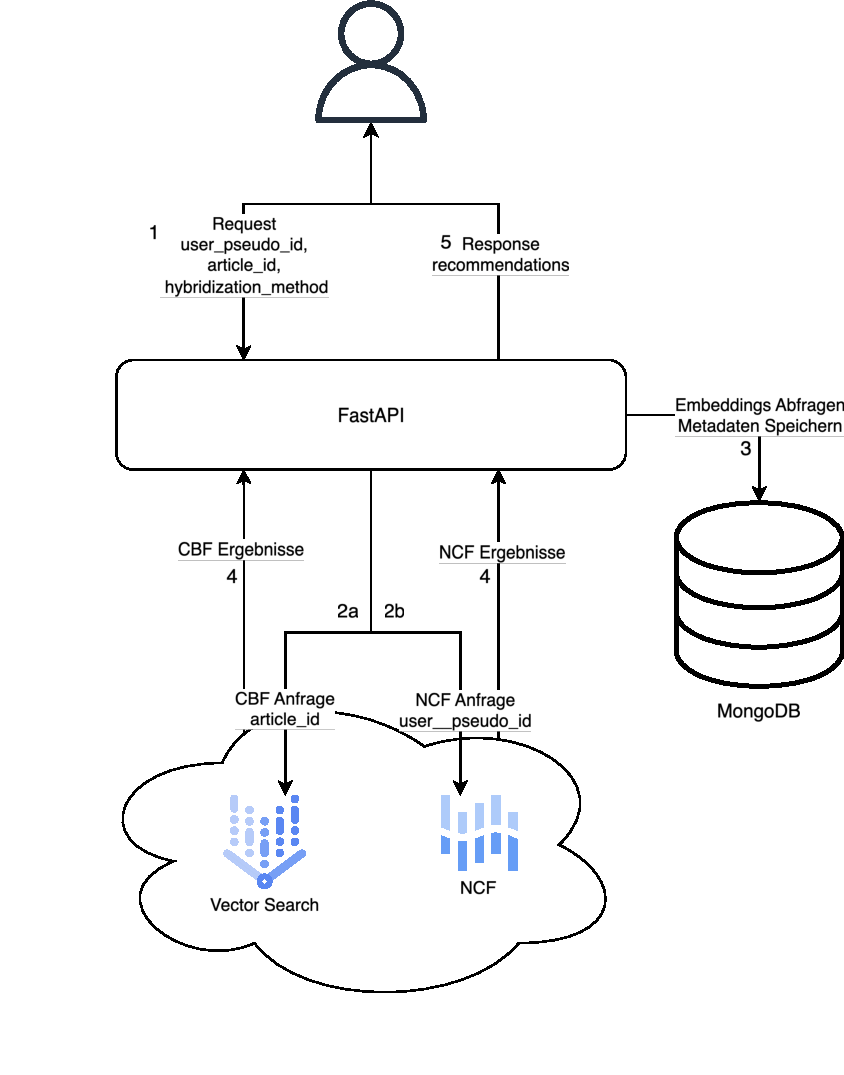
\includegraphics[width=0.6\textwidth]{content/figures/svg/architektur.pdf}
    \caption{Die technologische Architektur des hybriden Empfehlungssystems. Der nummerierte Datenfluss zeigt den Weg einer Anfrage vom Nutzer (1), 
    über die parallelen Abfragen an die ML-Dienste (2a, 2b) und die Datenbank (3), die eintreffenden Ergebnisse (4) bis zur finalen Empfehlung (5).}
    \label{fig:architektur}
\end{figure}
Die technologische Architektur ist als cloud-nativer Microservice-Ansatz auf der \ac{GCP} konzipiert,
um die in Abschnitt \ref{sec:nfr} definierten Anforderungen an Skalierbarkeit und Performanz zu erfüllen. 
Als zentraler Orchestrator dient ein in Python implementierter Service, der auf dem performanten FastAPI-Framework basiert. 
Dieser Service ist nicht nur für die Entgegennahme von Anfragen und die Steuerung der Modell-Endpunkte verantwortlich, 
sondern auch für die Hybridisierung der Empfehlungsergebnisse. Das Design wurde dabei modular gestaltet, 
um zukünftig auch fortgeschrittenere Hybridisierungsstrategien integrieren zu können.
\subsubsection{API und Orchestrirung}
\subsubsection{Content Based Filtering}
\subsubsection{NCF}
Als zugrunde liegende Technologie des \ac{CF} wird in dieser Arbeit \ac{NCF} verwendet. Dadurch wird in kurzer Zeit 
ein leistungsfähiges Modell bereitgestellt, welches zur Optimierung der Hybridisierungsstrategie verwendet werden kann.



\subsection{Datenbasis und Einschränkungen}
% 70.000 embedded Artikel
% GA4 Events: page_view, session_data
% Interaktionsmatrix